\documentclass[conference]{IEEEtran}
\IEEEoverridecommandlockouts

% Configuración para español
\usepackage[spanish,es-nodecimaldot,es-noshorthands]{babel}
\usepackage[utf8]{inputenc}
\usepackage[T1]{fontenc}

% Paquetes estándar IEEE
\usepackage{cite}
\usepackage{amsmath,amssymb,amsfonts}
\usepackage{algorithmic}
\usepackage{graphicx}
\usepackage{textcomp}
\usepackage{xcolor}
\usepackage{float}
\usepackage{listings} % Para código

% ---------- Configuración de listados de código ----------
\definecolor{codegray}{rgb}{0.45,0.45,0.45}
\definecolor{codeblue}{rgb}{0.10,0.10,0.60}
\lstset{
	basicstyle=\ttfamily\scriptsize,
	keywordstyle=\color{codeblue}\bfseries,
	commentstyle=\color{codegray}\itshape,
	stringstyle=\color{codegray},
	numbers=left,
	numberstyle=\tiny\color{codegray},
	numbersep=5pt,
	frame=single,
	breaklines=true,
	breakatwhitespace=true,
	showstringspaces=false,
	tabsize=2,
	captionpos=b,
	literate=%
	{á}{{\'a}}1 {é}{{\'e}}1 {í}{{\'i}}1 {ó}{{\'o}}1 {ú}{{\'u}}1
	{Á}{{\'A}}1 {É}{{\'E}}1 {Í}{{\'I}}1 {Ó}{{\'O}}1 {Ú}{{\'U}}1
	{ñ}{{\~n}}1 {Ñ}{{\~N}}1 {¿}{{?`}}1 {¡}{{!`}}1
}

% ---------- Espacio reservado para imágenes faltantes ----------
\newcommand{\imgph}[2]{%
	\fbox{\begin{minipage}[c][#2][c]{0.92\columnwidth}
			\centering\textcolor{codegray}{\footnotesize [Espacio para imagen: #1]}
	\end{minipage}}%
}

\def\BibTeX{{\rm B\kern-.05em{\sc i\kern-.025em b}\kern-.08em
	T\kern-.1667em\lower.7ex\hbox{E}\kern-.125emX}}

\begin{document}

\title{Práctica 1: Explorando Linux embebido en la Raspberry Pi}

\author{
	\IEEEauthorblockN{Belmont Muñoz Samuel}
	\IEEEauthorblockA{\textit{Ingeniería en Computación} \\
		\textit{Facultad de Ingeniería}\\
		No. Cuenta: 317318289}
	\and
	\IEEEauthorblockN{Domínguez Palacios Jesús Alejandro}
	\IEEEauthorblockA{\textit{Ingeniería en Computación} \\
		\textit{Facultad de Ingeniería}\\
		No. Cuenta: 421066205}
	\and
	\IEEEauthorblockN{Dorantes Mejía Emmanuel}
	\IEEEauthorblockA{\textit{Ingeniería en Computación} \\
		\textit{Facultad de Ingeniería}\\
		No. Cuenta: 313004766}
	\and
	\IEEEauthorblockN{García Olvera Emiliano}
	\IEEEauthorblockA{\textit{Ingeniería en Computación} \\
		\textit{Facultad de Ingeniería}\\
		No. Cuenta: 314256009}
	\and
	\IEEEauthorblockN{Hernández Alonso Antonio Adonahí}
	\IEEEauthorblockA{\textit{Ingeniería en Computación} \\
		\textit{Facultad de Ingeniería}\\
		No. Cuenta: 316339825}
	\and
	\IEEEauthorblockN{Jiménez Reyes Alan Yael}
	\IEEEauthorblockA{\textit{Ingeniería en Computación} \\
		\textit{Facultad de Ingeniería}\\
		No. Cuenta: 320026726}
}

\maketitle

\begin{center}
	\vspace{-0.3cm}
	{\small
		\textbf{Práctica No.:} 1 \quad | \quad
		\textbf{Grupo:} 6 \quad | \quad
		\textbf{Fecha:} 07/09/2026
	}
	\vspace{0.2cm}
\end{center}

\begin{abstract}
	Este reporte documenta la configuración del entorno de desarrollo en un sistema Linux embebido sobre Raspberry Pi 4 Model B Rev 1.5. Se describe la actualización del sistema operativo, la instalación de herramientas de compilación (toolchain), y la creación de programas en C y scripts de Bash para diagnóstico del sistema. El documento aborda la gestión de paquetes con APT, la inspección de configuraciones de bajo nivel a través de \texttt{/proc} y \texttt{/sys}, y el uso de Git para control de versiones. Se incluye el desarrollo de un programa que extrae información real del hardware y un script automatizado de monitoreo del sistema.
\end{abstract}

\begin{IEEEkeywords}
	Linux embebido, Raspberry Pi, toolchain, gcc, Git, scripts Bash, programación en C
\end{IEEEkeywords}

\section{Objetivo}
Los objetivos de esta práctica son:
\begin{itemize}
	\item Actualizar el sistema y gestionar paquetes con APT.
	\item Instalar y verificar gcc, make y git.
	\item Inspeccionar la configuración de arranque y el árbol de dispositivos.
	\item Escribir un programa en C que reporte arquitectura, CPU y memoria reales del sistema.
	\item Combinar comandos de diagnóstico en un script de Bash.
	\item Registrar el primer commit de Git en un repositorio que se usará el resto del semestre.
\end{itemize}

Al finalizar la práctica se debe tener: el programa \texttt{reporte\_sistema} compilando y mostrando datos reales, el script \texttt{sysinfo} con permiso de ejecución y su archivo de registro generado, y el historial de Git mostrando al menos un commit.

\section{Introducción}
El desarrollo de aplicaciones para sistemas embebidos requiere un entorno de trabajo adecuadamente configurado con herramientas de compilación, depuración y control de versiones. En sistemas Linux embebidos como Raspberry Pi OS, estas herramientas conforman lo que se conoce como \textit{toolchain} de desarrollo \cite{gnu_toolchain}.

Un toolchain típico incluye el compilador GCC (\textit{GNU Compiler Collection}) para transformar código fuente en ejecutables nativos, Make para automatizar el proceso de compilación mediante archivos Makefile, y Git para el control de versiones distribuido del código fuente. Estas herramientas son fundamentales en el flujo de trabajo de desarrollo embebido profesional.

La gestión de paquetes en Raspberry Pi OS se realiza mediante APT (\textit{Advanced Package Tool}), el sistema de administración de software heredado de Debian. APT permite instalar, actualizar y eliminar software de repositorios oficiales y comunitarios, manteniendo el sistema actualizado con parches de seguridad y nuevas funcionalidades.

En cuanto a la inspección del sistema a bajo nivel, Linux expone información de hardware y configuración del kernel a través de los sistemas de archivos virtuales \texttt{/proc} y \texttt{/sys} \cite{linux_proc}. Archivos como \texttt{/proc/cpuinfo}, \texttt{/proc/meminfo} y \texttt{/boot/firmware/config.txt} proporcionan datos esenciales sobre el procesador, memoria y configuración de arranque. El árbol de dispositivos (\textit{Device Tree}) es un mecanismo utilizado en arquitecturas ARM para describir el hardware disponible al kernel durante el arranque \cite{rpi_docs}.

La programación en C sigue siendo el lenguaje dominante en sistemas embebidos debido a su cercanía al hardware, eficiencia y portabilidad. La capacidad de leer archivos del sistema virtual permite que programas en C obtengan información dinámica del hardware sin depender de bibliotecas externas pesadas.

Por otro lado, los scripts de Bash automatizan tareas administrativas y de diagnóstico. Un script bien diseñado puede ejecutar comandos del sistema, procesar su salida y generar reportes, todo de forma reproducible y documentada \cite{bash_guide}.

\section{Desarrollo}

\subsection{Material y Equipo}
Para la realización de esta práctica se utilizaron los siguientes elementos:
\begin{itemize}
	\item Raspberry Pi 4 Model B Rev 1.5 con Raspberry Pi OS (base Debian \textit{trixie}), kernel \texttt{6.18.39+rpt-rpi-v8}, con nombre de host \texttt{konan}
	\item Fuente de alimentación USB-C y tarjeta microSD de 64~GB con el sistema instalado en la Práctica 0
	\item Computadora host con cliente SSH
	\item Conexión a Internet para la descarga de paquetes
\end{itemize}

El trabajo se organizó rotando los roles de \textit{piloto} (escribe y ejecuta los comandos) y \textit{copiloto} (lee el paso, verifica la salida y registra las diferencias) en cada una de las siete partes de la práctica.

\subsection{Procedimiento}

\subsubsection{Parte A: Actualización del sistema y toolchain}
Se estableció la conexión remota por SSH desde la computadora host hacia la Raspberry Pi, usando el nombre de host configurado en la Práctica 0. Ya dentro de la sesión, se actualizó el índice de paquetes y posteriormente el sistema completo.

\begin{lstlisting}[language=bash,caption={Actualización del sistema con APT.}]
sudo apt update
sudo apt upgrade -y
\end{lstlisting}

El primer comando descarga las listas de paquetes desde los repositorios configurados; el segundo instala las versiones nuevas de los paquetes ya presentes en el sistema. La bandera \texttt{-y} evita la confirmación interactiva.

\begin{figure}[H]
	\centering
	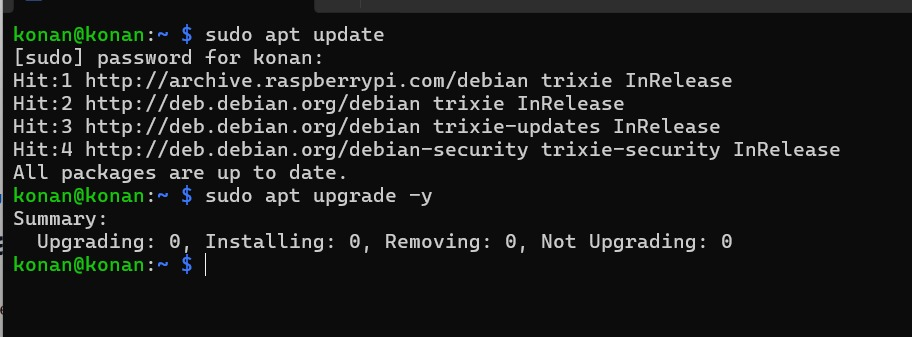
\includegraphics[width=\columnwidth]{img/fig01_apt.png}
	\caption{Actualización del índice de paquetes y del sistema mediante APT.}
	\label{fig:apt}
\end{figure}

Enseguida se instaló el toolchain de desarrollo en C junto con el sistema de control de versiones. El metapaquete \texttt{build-essential} agrupa el compilador GCC, las bibliotecas estándar de desarrollo y la utilidad \texttt{make}.

\begin{lstlisting}[language=bash,caption={Instalación y verificación del toolchain.}]
sudo apt install -y build-essential git

gcc --version
make --version
git --version
\end{lstlisting}

\begin{figure}[H]
	\centering
	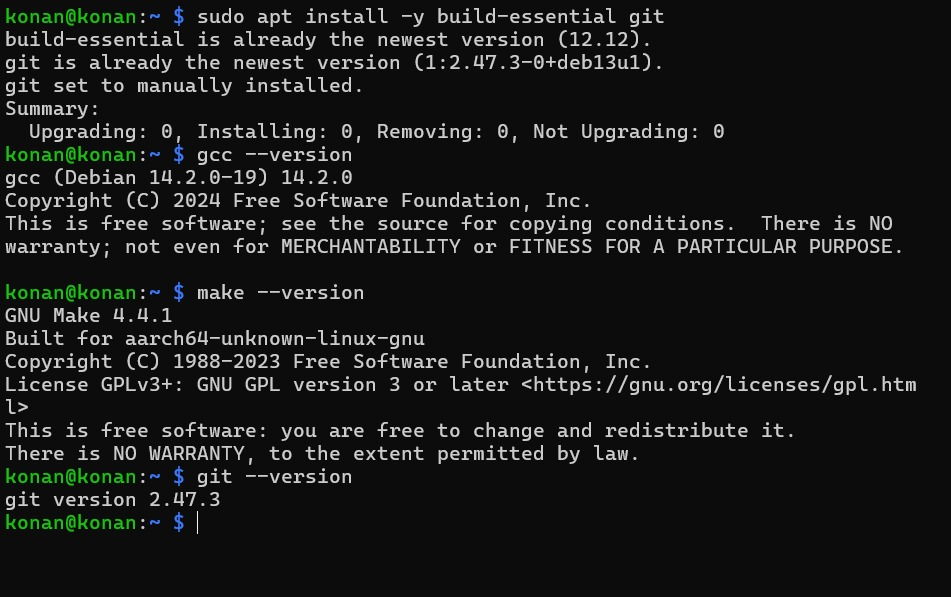
\includegraphics[width=\columnwidth]{img/fig02_toolchain.png}
	\caption{Instalación del toolchain y verificación de las versiones de gcc, make y git.}
	\label{fig:toolchain}
\end{figure}

\subsubsection{Parte B: Configuración de arranque y árbol de dispositivos}
Se inspeccionó el archivo de configuración de arranque, que en las versiones de Raspberry Pi OS basadas en Bookworm y posteriores reside en \texttt{/boot/firmware/config.txt} (en versiones anteriores la ruta era \texttt{/boot/config.txt}). Este archivo lo lee el firmware antes de que el kernel tome el control, y en él se declaran parámetros como los \textit{overlays} del árbol de dispositivos, la habilitación de interfaces (I\textsuperscript{2}C, SPI, UART) y la configuración de video.

\begin{lstlisting}[language=bash,caption={Inspección de la partición de arranque.}]
cat /boot/firmware/config.txt
ls /boot/firmware/
\end{lstlisting}



\begin{figure}[H]
	\centering
	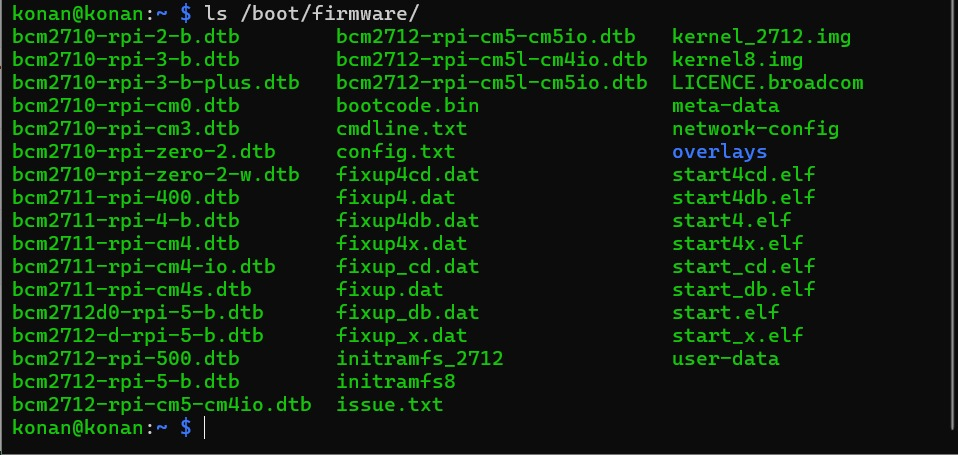
\includegraphics[width=\columnwidth]{img/fig04_bootfirmware.png}
	\caption{Contenido de la partición de arranque: firmware del GPU, imágenes del kernel y archivos \texttt{.dtb} de árbol de dispositivos.}
	\label{fig:bootdir}
\end{figure}

Posteriormente se exploró la representación en vivo del árbol de dispositivos, es decir, la versión ya cargada e interpretada por el kernel y expuesta como sistema de archivos virtual.

\begin{lstlisting}[language=bash,caption={Exploración del device tree activo.}]
ls /proc/device-tree/
\end{lstlisting}

\begin{figure}[H]
	\centering
	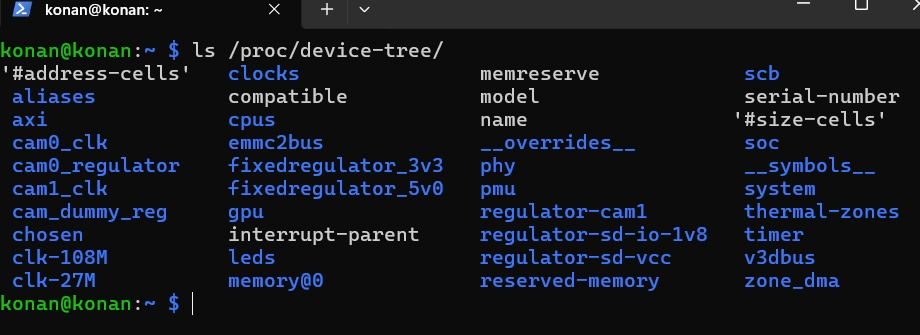
\includegraphics[width=\columnwidth]{img/fig05_devicetree.png}
	\caption{Nodos del árbol de dispositivos detectados por el kernel.}
	\label{fig:devicetree}
\end{figure}

\subsubsection{Parte C: Procesos y servicios}
Para observar los procesos activos se emplearon dos herramientas complementarias: \texttt{ps aux}, que entrega una fotografía estática de todos los procesos del sistema, y \texttt{top}, que muestra la misma información actualizándose en tiempo real y ordenada por consumo de CPU.

\begin{lstlisting}[language=bash,caption={Inspección de procesos activos.}]
ps aux
top
\end{lstlisting}

\begin{figure}[H]
	\centering
	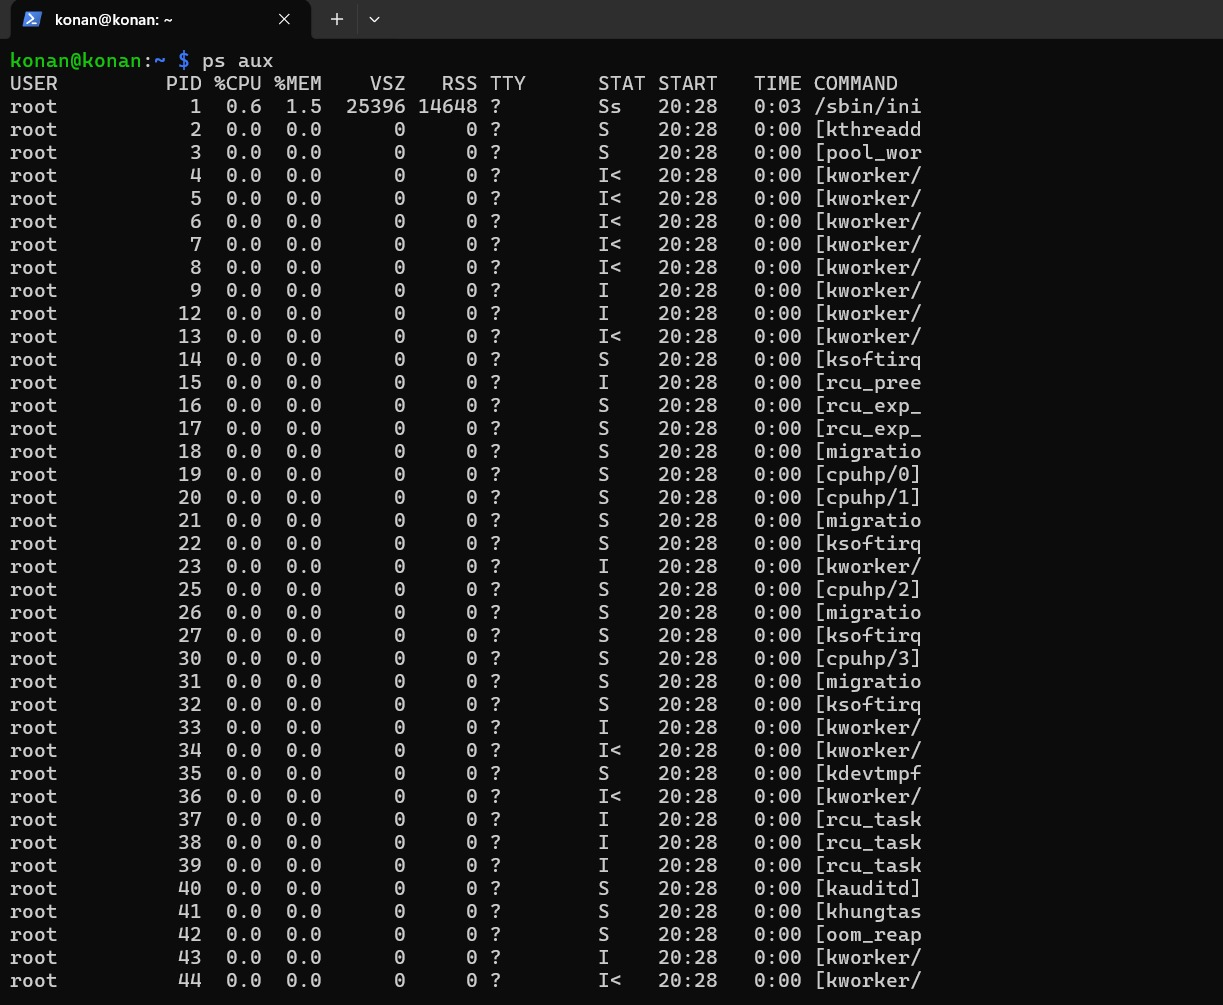
\includegraphics[width=\columnwidth]{img/fig06_psaux.png}
	\caption{Listado de procesos activos con \texttt{ps aux}.}
	\label{fig:psaux}
\end{figure}

\begin{figure}[H]
	\centering
	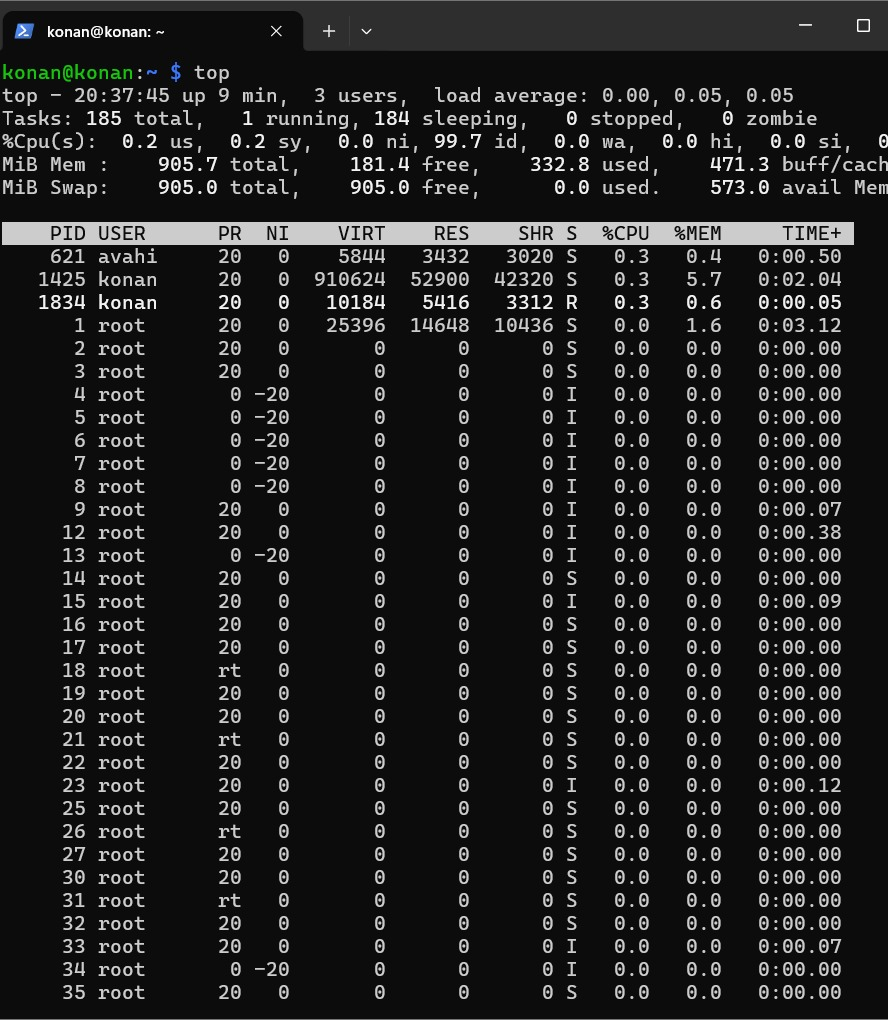
\includegraphics[width=\columnwidth]{img/fig07_top.png}
	\caption{Monitor de procesos en tiempo real \texttt{top}, con el resumen de tareas, uso de CPU y memoria.}
	\label{fig:top}
\end{figure}

Finalmente se revisó el estado del gestor de servicios \texttt{systemd}, responsable de arrancar y supervisar los servicios del sistema.

\begin{lstlisting}[language=bash,caption={Revisión de servicios del sistema.}]
systemctl status
systemctl list-units --type=service | head -n 15
\end{lstlisting}

\begin{figure}[H]
	\centering
	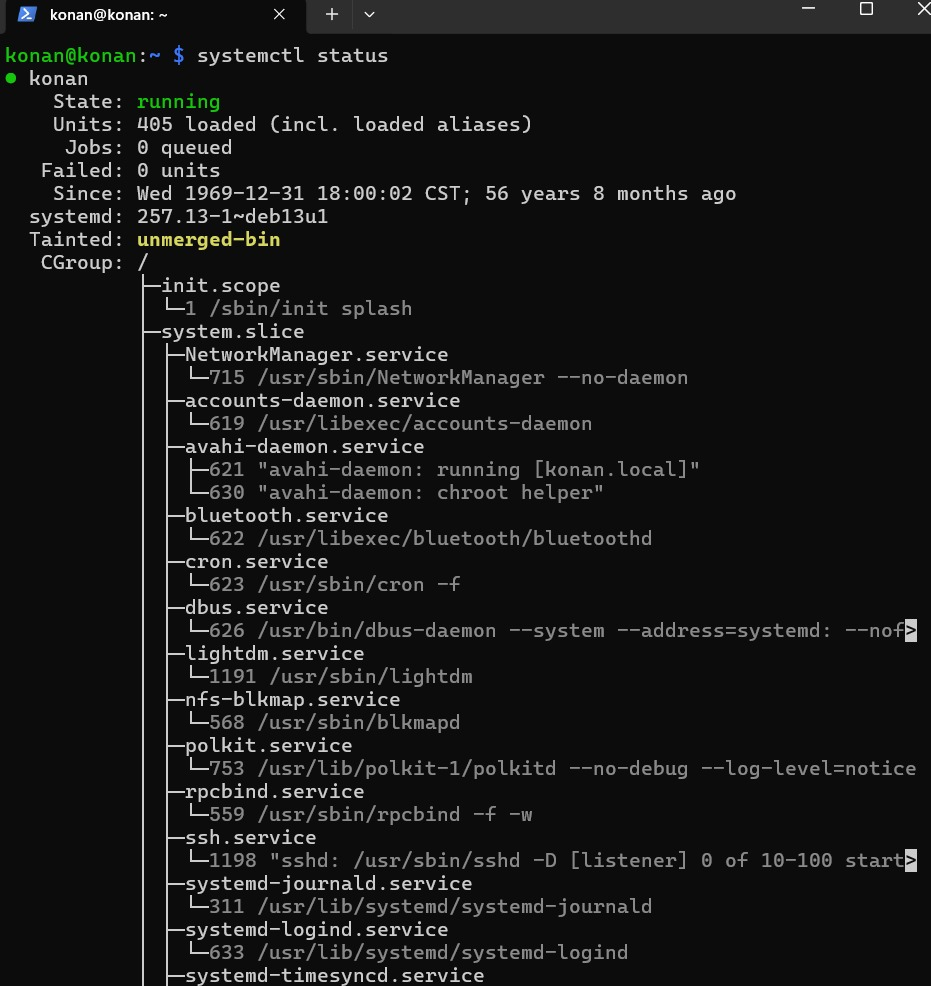
\includegraphics[width=\columnwidth]{img/fig08_systemctl_status.png}
	\caption{Estado general del sistema y árbol de grupos de control reportado por \texttt{systemd}.}
	\label{fig:systemctl}
\end{figure}

\begin{figure}[H]
	\centering
	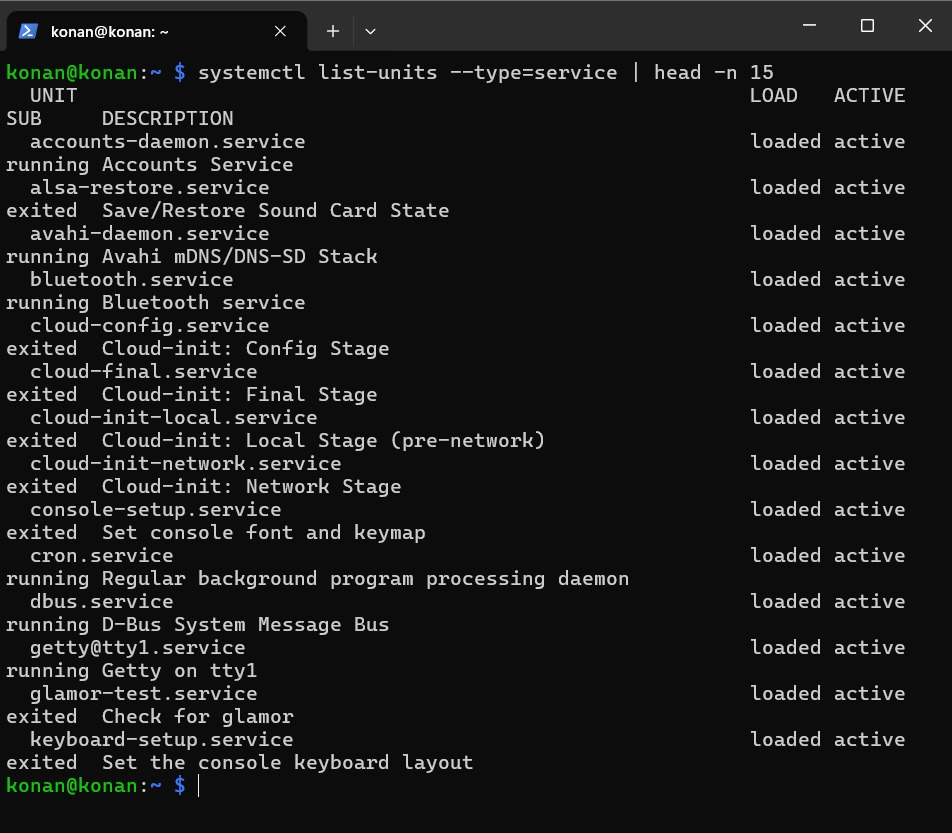
\includegraphics[width=\columnwidth]{img/fig09_systemctl_units.png}
	\caption{Primeras quince unidades de tipo servicio con su estado de carga y actividad.}
	\label{fig:units}
\end{figure}

\subsubsection{Parte D: Programa en C de reporte del sistema}
Se escribió el programa \texttt{reporte\_sistema.c}, que obtiene información del sistema por dos vías distintas: la llamada \texttt{uname()} de la biblioteca estándar, que entrega arquitectura y versión del kernel a través de la estructura \texttt{struct utsname}, y la lectura directa de los archivos virtuales \texttt{/proc/cpuinfo} y \texttt{/proc/meminfo}.

Para evitar duplicar código en la lectura de ambos archivos se implementó la función auxiliar \texttt{mostrar\_linea()}, que recorre un archivo abierto línea por línea con \texttt{fgets()} y compara el inicio de cada línea contra una etiqueta usando \texttt{strncmp()}. Al encontrar la primera coincidencia la imprime y termina la búsqueda. Para el reto opcional se agregó la función \texttt{valor\_kb()}, que en lugar de imprimir la línea completa extrae con \texttt{sscanf()} el valor numérico asociado a la etiqueta y lo devuelve como \texttt{long}, o \texttt{-1} si no la encuentra.

\begin{lstlisting}[language=C,caption={Código fuente de \texttt{reporte\_sistema.c}.}]
#include <stdio.h>
#include <string.h>
#include <sys/utsname.h>

/* Busca la primera linea que empiece con 'etiqueta' y la imprime. */
void mostrar_linea(FILE *f, const char *etiqueta) {
	char linea[256];
	while (fgets(linea, sizeof(linea), f)) {
		if (strncmp(linea, etiqueta, strlen(etiqueta)) == 0) {
			printf("%s", linea);
			break;
		}
	}
}

/* Reto opcional: devuelve el valor numerico (en kB) de una etiqueta
   de /proc/meminfo, o -1 si no la encuentra. */
long valor_kb(FILE *f, const char *etiqueta) {
	char linea[256];
	long valor;
	while (fgets(linea, sizeof(linea), f)) {
		if (strncmp(linea, etiqueta, strlen(etiqueta)) == 0) {
			if (sscanf(linea + strlen(etiqueta), " : %ld", &valor) == 1)
				return valor;
		}
	}
	return -1;
}

int main(void) {
	struct utsname info;
	uname(&info);

	printf("=== Reporte del sistema ===\n");
	printf("Arquitectura: %s\n", info.machine);
	printf("Kernel:       %s\n", info.release);

	FILE *cpu = fopen("/proc/cpuinfo", "r");
	if (cpu) {
		printf("\n-- CPU --\n");
		mostrar_linea(cpu, "Model");
		mostrar_linea(cpu, "Hardware");
		fclose(cpu);
	}

	FILE *mem = fopen("/proc/meminfo", "r");
	if (mem) {
		printf("\n-- Memoria --\n");
		mostrar_linea(mem, "MemTotal");
		mostrar_linea(mem, "MemFree");
		rewind(mem);
		long libre = valor_kb(mem, "MemFree");
		if (libre >= 0)
			printf("Memoria libre: %.1f MB\n", libre / 1024.0);
		fclose(mem);
	}

	return 0;
}
\end{lstlisting}

\begin{figure}[H]
	\centering
	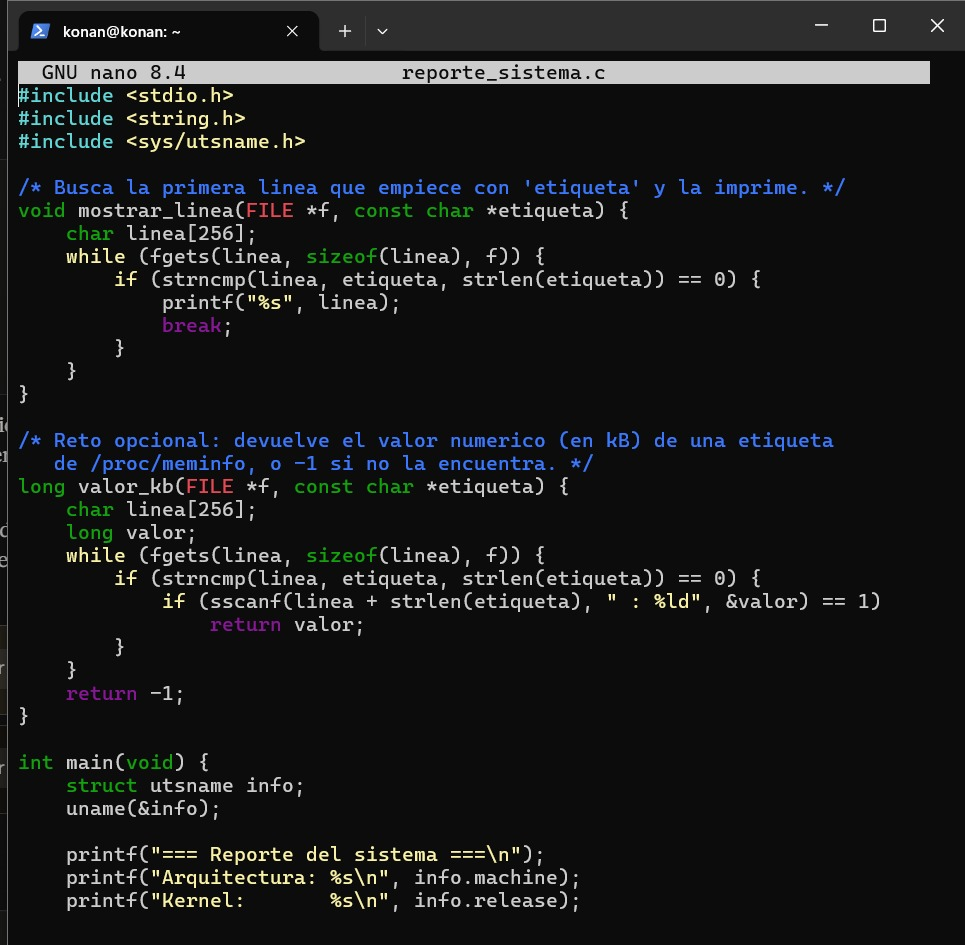
\includegraphics[width=\columnwidth]{img/fig10_codigo_c.png}
	\caption{Edición del programa \texttt{reporte\_sistema.c} en el editor \texttt{nano}.}
	\label{fig:codigoc}
\end{figure}

La compilación y ejecución se realizaron con:

\begin{lstlisting}[language=bash,caption={Compilación y ejecución del programa.}]
gcc reporte_sistema.c -o reporte_sistema
./reporte_sistema
\end{lstlisting}

\begin{figure}[H]
	\centering
	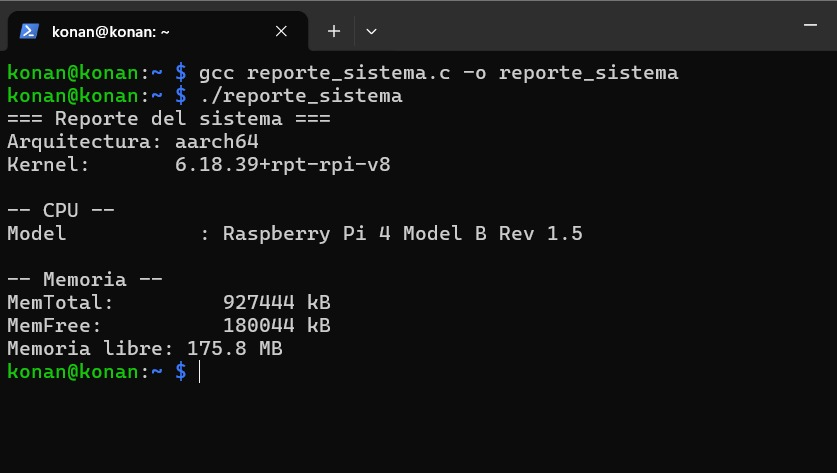
\includegraphics[width=\columnwidth]{img/fig11_salida_reporte.png}
	\caption{Salida del programa \texttt{reporte\_sistema} con datos reales del hardware.}
	\label{fig:reporte}
\end{figure}

\subsubsection{Parte E: GPIO por software}
Sin conectar hardware externo, se verificó que el kernel siguiera exponiendo la interfaz de propósito general de entrada/salida a través del sistema de archivos \texttt{sysfs}.

\begin{lstlisting}[language=bash,caption={Verificación de la interfaz GPIO.}]
ls /sys/class/gpio/
\end{lstlisting}

\begin{figure}[H]
	\centering
	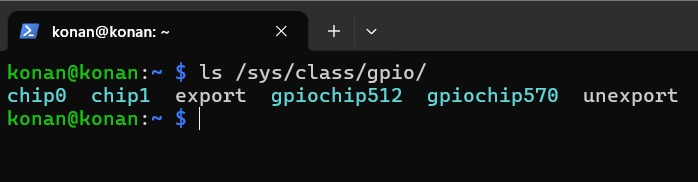
\includegraphics[width=\columnwidth]{img/fig12_gpio.png}
	\caption{Interfaz GPIO expuesta por el kernel en \texttt{sysfs}.}
	\label{fig:gpio}
\end{figure}

\subsubsection{Parte F: Script de diagnóstico en Bash}
Se creó el script \texttt{sysinfo.sh}, que agrupa varios de los comandos de diagnóstico utilizados durante la práctica y guarda la salida completa en un archivo de registro con marca de tiempo en el nombre. El bloque de comandos se agrupa entre llaves y se canaliza hacia \texttt{tee}, lo que permite mostrar la salida en pantalla y escribirla en el archivo simultáneamente.

\begin{lstlisting}[language=bash,caption={Código fuente de \texttt{sysinfo.sh}.}]
#!/bin/bash
LOG="sysinfo_$(date +%Y%m%d_%H%M%S).log"
{
	echo "=== Reporte generado el $(date) ==="
	echo "--- Sistema ---"; uname -a
	echo "--- CPU ---";     lscpu | head -n 10
	echo "--- Memoria ---"; free -h
	echo "--- Disco ---";   df -h /
	echo "--- Procesos ---"; ps aux --sort=-%cpu | head -n 6
} | tee "$LOG"
echo "Reporte guardado en: $LOG"
\end{lstlisting}

\begin{figure}[H]
	\centering
	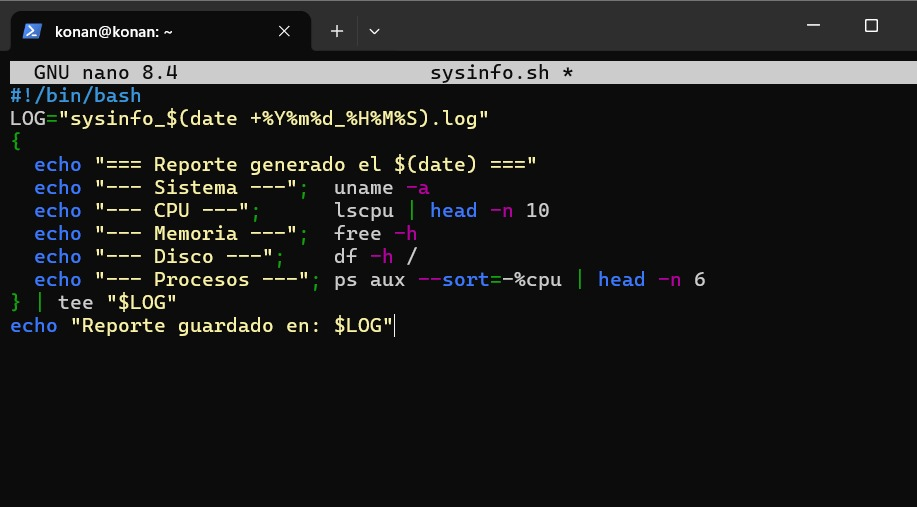
\includegraphics[width=\columnwidth]{img/fig13_script_bash.png}
	\caption{Edición del script \texttt{sysinfo.sh} en \texttt{nano}.}
	\label{fig:scriptbash}
\end{figure}

Como el archivo se crea sin permiso de ejecución, fue necesario otorgarlo antes de correrlo:

\begin{lstlisting}[language=bash,caption={Permisos y ejecución del script.}]
chmod +x sysinfo.sh
./sysinfo.sh
cat sysinfo_*.log
\end{lstlisting}

\begin{figure}[H]
	\centering
	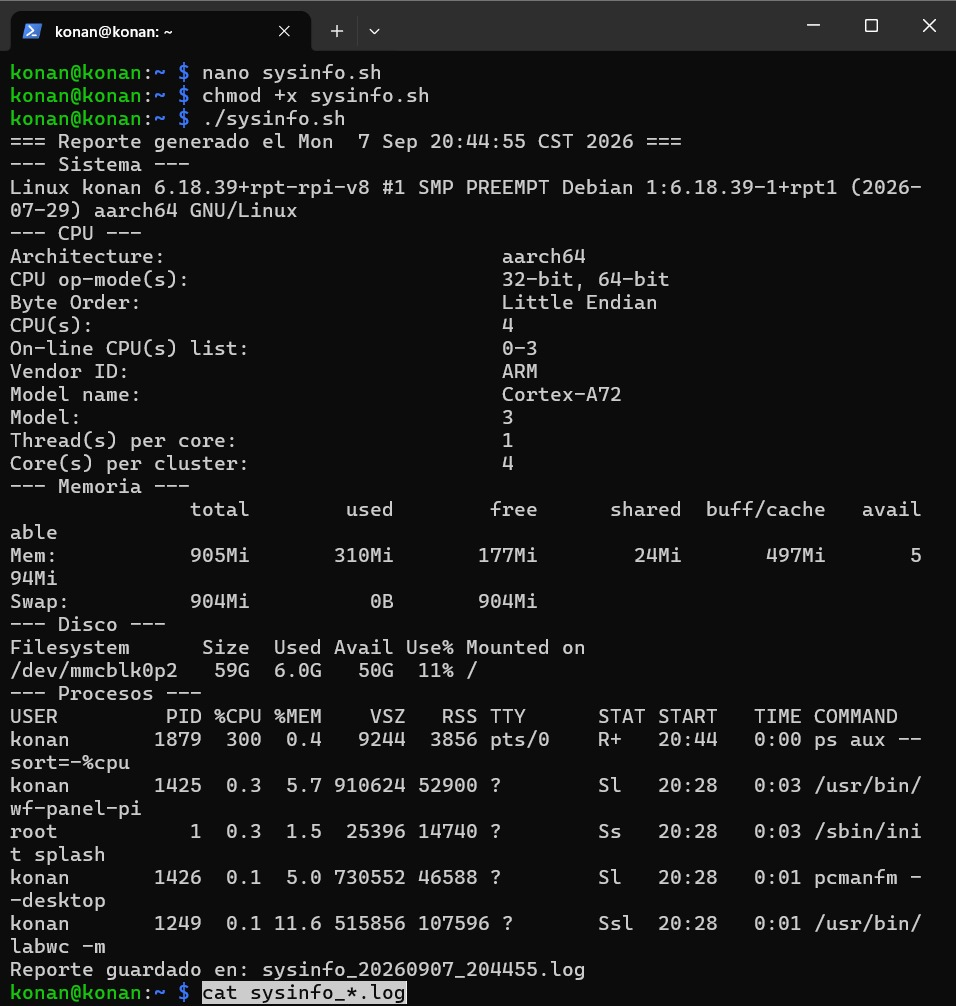
\includegraphics[width=\columnwidth]{img/fig14_sysinfo_exec.png}
	\caption{Ejecución del script tras otorgar el permiso de ejecución.}
	\label{fig:sysinfoexec}
\end{figure}

\begin{figure}[H]
	\centering
	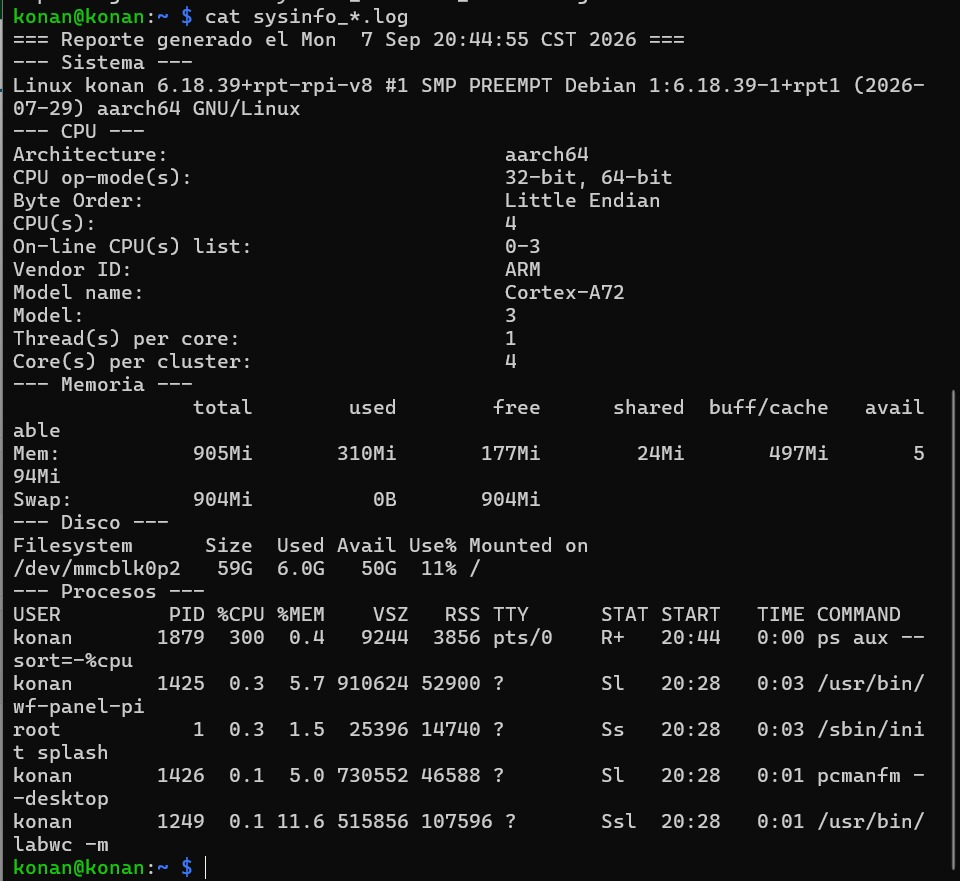
\includegraphics[width=\columnwidth]{img/fig15_sysinfo_log.png}
	\caption{Contenido del archivo de registro \texttt{sysinfo\_20260907\_204455.log} generado por el script.}
	\label{fig:sysinfolog}
\end{figure}

\subsubsection{Parte G: Primer commit con Git}
Se configuró la identidad del usuario a nivel global en la Raspberry Pi, requisito indispensable para que Git pueda firmar los commits. El repositorio se creó dentro del directorio \texttt{\textasciitilde/fse}, que será el mismo que se utilice en las prácticas siguientes.

\begin{lstlisting}[language=bash,caption={Configuración de identidad e inicialización del repositorio.}]
git config --global user.name "J Alejandro Dominguez"
git config --global user.email "adp3993@gmail.com"

git init
git add reporte_sistema.c sysinfo.sh
git commit -m "Practica 1"
git log
\end{lstlisting}

Se agregaron al área de preparación únicamente los archivos fuente producidos durante la sesión, dejando fuera el binario compilado y los archivos de registro, ya que son artefactos regenerables. Dado que el primer commit se realizó antes de terminar de configurar el correo electrónico, se corrigió la autoría y se amplió el mensaje con los nombres del equipo mediante:

\begin{lstlisting}[language=bash,caption={Corrección de autoría del commit.}]
git commit --amend --reset-author -m "Practica 1

Belmont Munoz Samuel
Dominguez Palacios Jesus Alejandro
Dorantes Mejia Emmanuel
Garcia Olvera Emiliano
Hernandez Alonso Antonio Adonahi
Jimenez Reyes Alan Yael"
\end{lstlisting}

\begin{figure}[H]
	\centering
	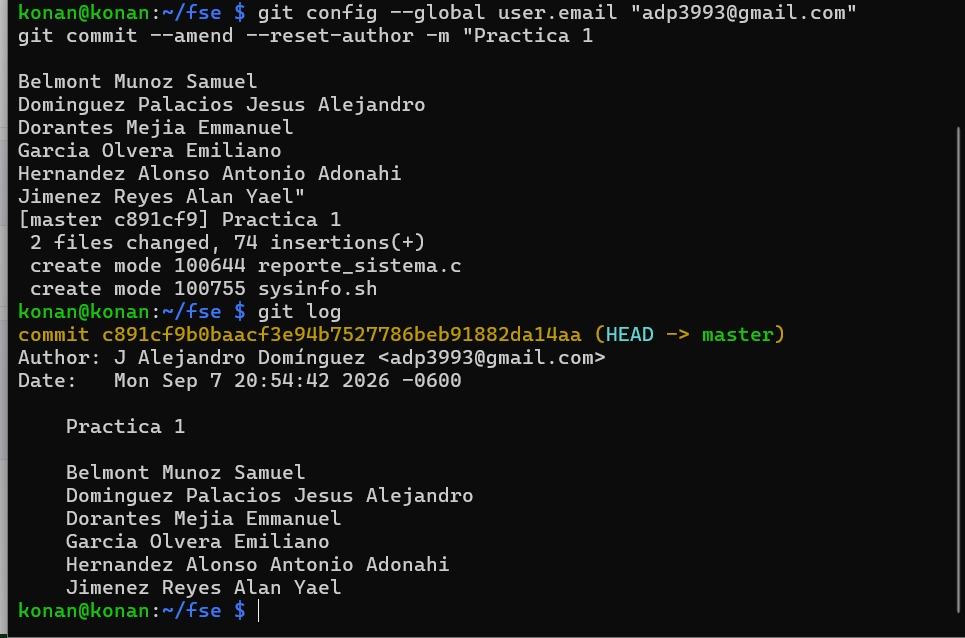
\includegraphics[width=\columnwidth]{img/fig16_gitlog.png}
	\caption{Corrección de autoría e historial del repositorio mostrando el commit \texttt{c891cf9}.}
	\label{fig:gitlog}
\end{figure}

\section{Resultados y Análisis}

\subsection{Actualización y toolchain}
El comando \texttt{apt update} contactó cuatro repositorios: el de Raspberry Pi (\texttt{archive.raspberrypi.com/debian trixie}) y tres de Debian (\texttt{trixie}, \texttt{trixie-updates} y \texttt{trixie-security}), reportando que todos los paquetes ya estaban al día. En consecuencia, \texttt{apt upgrade -y} resumió cero paquetes actualizados, instalados o eliminados (Fig.~\ref{fig:apt}). El sistema ya se encontraba actualizado desde la instalación realizada en la Práctica 0.

De forma análoga, \texttt{build-essential} (versión 12.12) y \texttt{git} (1:2.47.3-0+deb13u1) ya estaban instalados, por lo que APT únicamente los marcó como instalados manualmente. Las versiones verificadas se resumen en la Tabla~\ref{tab:toolchain}.

\begin{table}[H]
	\centering
	\caption{Versiones del toolchain instalado.}
	\label{tab:toolchain}
	\begin{tabular}{|l|l|}
		\hline
		\textbf{Herramienta} & \textbf{Versión} \\
		\hline
		GCC & 14.2.0 (Debian 14.2.0-19) \\
		\hline
		GNU Make & 4.4.1 \\
		\hline
		Git & 2.47.3 \\
		\hline
		build-essential & 12.12 \\
		\hline
	\end{tabular}
\end{table}

Un detalle relevante es la línea \textit{Built for aarch64-unknown-linux-gnu} que reporta Make: confirma que las herramientas fueron compiladas para la misma arquitectura sobre la que se ejecutan. Se trata entonces de compilación nativa, donde el mismo equipo que ejecuta el programa lo genera. Esto contrasta con el esquema de compilación cruzada usado en microcontroladores sin sistema operativo, donde el binario se produce en una máquina host de arquitectura distinta y luego se transfiere al dispositivo.

\subsection{Arranque y árbol de dispositivos}
El listado de \texttt{/boot/firmware/} (Fig.~\ref{fig:bootdir}) reveló que la partición de arranque no contiene únicamente los archivos de este modelo, sino los de toda la familia. Se identificaron tres grupos de archivos \texttt{.dtb}: los \texttt{bcm2710-*} (Raspberry Pi 3 y Zero 2 W), los \texttt{bcm2711-*} (Pi 4, Pi 400 y CM4) y los \texttt{bcm2712-*} (Pi 5, Pi 500 y CM5). Junto a ellos aparecen dos imágenes de kernel, \texttt{kernel8.img} y \texttt{kernel\_2712.img}, y el firmware propietario del GPU (\texttt{bootcode.bin}, los archivos \texttt{start*.elf} y sus correspondientes \texttt{fixup*.dat}).

Esto explica el mecanismo real de arranque: una sola imagen de tarjeta sirve para varios modelos porque el firmware, al iniciar, identifica la revisión de la placa y selecciona el \texttt{.dtb} y la imagen de kernel correctos. También se observó el directorio \texttt{overlays/}, que contiene los fragmentos de árbol de dispositivos que \texttt{config.txt} puede activar para habilitar periféricos opcionales, y los archivos \texttt{meta-data}, \texttt{network-config} y \texttt{user-data}, propios del mecanismo de aprovisionamiento \textit{cloud-init}.

El listado de \texttt{/proc/device-tree/} (Fig.~\ref{fig:devicetree}) confirmó que el kernel interpretó ese descriptor binario y expuso cada nodo como un directorio navegable. Entre los nodos se identificaron \texttt{model} y \texttt{compatible}, que identifican la placa; \texttt{cpus} y \texttt{memory@0}, que declaran los recursos de cómputo y memoria; \texttt{soc}, que agrupa los periféricos integrados; y nodos de hardware específico como \texttt{gpu}, \texttt{v3dbus}, \texttt{leds}, \texttt{thermal-zones}, \texttt{timer}, los reguladores fijos \texttt{fixedregulator\_3v3} y \texttt{fixedregulator\_5v0}, y los relojes y reguladores de las interfaces de cámara (\texttt{cam0\_clk}, \texttt{cam1\_clk}, \texttt{regulator-cam1}).

Esto ilustra de forma concreta el concepto de BSP visto en la Unidad 2: en ARM el kernel no descubre el hardware por enumeración automática, como ocurre en PCI o USB, sino que recibe su descripción explícita en el momento del arranque. Los nodos \texttt{\_\_symbols\_\_} y \texttt{\_\_overrides\_\_} son precisamente los puntos de anclaje que permiten a los overlays modificar ese árbol sin recompilarlo por completo.

\subsection{Procesos y servicios}
La salida de \texttt{ps aux} (Fig.~\ref{fig:psaux}) mostró en la primera posición el proceso con PID 1, \texttt{/sbin/init splash}, que en este sistema es \texttt{systemd} y actúa como ancestro de todos los procesos de usuario. Inmediatamente después aparece una larga secuencia de procesos cuyos nombres están entre corchetes (\texttt{[kthreadd]}, \texttt{[kworker/...]}, \texttt{[ksoftirqd]}, \texttt{[migration]}, \texttt{[rcu\_...]}) y cuyas columnas \texttt{VSZ} y \texttt{RSS} valen cero. Son hilos del kernel: se planifican como cualquier otro proceso, pero no tienen espacio de direcciones de usuario, por lo que no ocupan memoria virtual propia.

Los estados observados en la columna \texttt{STAT} fueron principalmente \texttt{S} (\textit{sleeping}, equivalente al estado bloqueado del diagrama visto en clase), \texttt{I} e \texttt{I<} (hilos de kernel ociosos, el segundo con prioridad elevada por \textit{nice} negativo), \texttt{R} (en ejecución) y \texttt{Ss} (en espera, además líder de sesión).

El monitor \texttt{top} (Fig.~\ref{fig:top}) cuantificó esa observación de manera contundente: de 185 tareas totales, 184 estaban durmiendo y solamente 1 en ejecución, sin procesos detenidos ni zombis, con el CPU 99.7\% inactivo y un \textit{load average} de 0.00. El único proceso en estado \texttt{R} era el propio \texttt{top}. Este es el comportamiento normal de un sistema multitarea: la inmensa mayoría de los procesos permanece bloqueada esperando un evento, y el planificador solo necesita repartir el CPU entre los pocos que están listos.

En cuanto a memoria, \texttt{top} reportó 905.7~MiB totales, con 181.4~MiB libres, 332.8~MiB en uso y 471.3~MiB en \textit{buffers} y caché, además de 905.0~MiB de espacio de intercambio completamente sin utilizar. Vale la pena notar que la memoria dedicada a caché no está desperdiciada: el kernel la libera automáticamente cuando una aplicación la necesita, razón por la cual la métrica \textit{available} (573.0~MiB) es más significativa que \textit{free}.

El comando \texttt{systemctl status} (Fig.~\ref{fig:systemctl}) reportó el sistema en estado \textit{running}, con 405 unidades cargadas, cero trabajos en cola y cero unidades fallidas, bajo \texttt{systemd} 257.13. En el árbol de grupos de control se distinguen \texttt{init.scope}, que contiene al PID 1, y \texttt{system.slice}, que agrupa los servicios del sistema: \texttt{NetworkManager}, \texttt{ssh} (con \texttt{sshd} escuchando conexiones, que es justamente el servicio que hace posible esta sesión de trabajo), \texttt{avahi-daemon} anunciando el nombre \texttt{konan.local} por mDNS, \texttt{bluetooth}, \texttt{cron}, \texttt{dbus}, \texttt{lightdm}, \texttt{polkit}, \texttt{systemd-journald}, \texttt{systemd-logind} y \texttt{systemd-timesyncd}.

Un dato llamativo fue la marca temporal de arranque: \textit{Since: Wed 1969-12-31 18:00:02 CST}. La Raspberry Pi carece de reloj de tiempo real con batería, por lo que al encender parte del inicio de la época Unix (1 de enero de 1970 UTC, que en la zona horaria local CST corresponde al 31 de diciembre de 1969 a las 18:00) hasta que \texttt{systemd-timesyncd} sincroniza la hora por NTP. En un sistema embebido sin conexión de red permanente, esta limitación obliga a incluir un módulo RTC externo si la aplicación depende de marcas de tiempo confiables.

Finalmente, el listado de unidades de servicio (Fig.~\ref{fig:units}) evidenció la diferencia entre los subestados \texttt{running} y \texttt{exited}. Servicios como \texttt{cron.service} o \texttt{dbus.service} permanecen en \texttt{running} porque mantienen un demonio vivo; en cambio \texttt{alsa-restore.service}, \texttt{console-setup.service}, \texttt{keyboard-setup.service} y las cuatro etapas de \texttt{cloud-init} aparecen como \texttt{active (exited)}: son servicios de tipo \textit{oneshot} que ejecutaron su tarea de configuración y terminaron, pero \texttt{systemd} los mantiene marcados como activos para registrar que ya se cumplieron.

\subsection{Programa en C}
El programa \texttt{reporte\_sistema} compiló sin advertencias ni errores y produjo los valores de la Tabla~\ref{tab:reporte} (Fig.~\ref{fig:reporte}).

\begin{table}[H]
	\centering
	\caption{Datos obtenidos por \texttt{reporte\_sistema}.}
	\label{tab:reporte}
	\begin{tabular}{|l|l|}
		\hline
		\textbf{Campo} & \textbf{Valor obtenido} \\
		\hline
		Arquitectura & \texttt{aarch64} \\
		\hline
		Kernel & \texttt{6.18.39+rpt-rpi-v8} \\
		\hline
		Model & Raspberry Pi 4 Model B Rev 1.5 \\
		\hline
		MemTotal & 927\,444 kB \\
		\hline
		MemFree & 180\,044 kB \\
		\hline
		Memoria libre & 175.8 MB \\
		\hline
	\end{tabular}
\end{table}

Los valores coincidieron con los obtenidos previamente mediante los comandos del sistema. El total de 927\,444~kB equivale a 905.7~MiB, exactamente la cifra que reportó \texttt{top} como memoria total, y la arquitectura \texttt{aarch64} es la misma que declaró \texttt{lscpu}. Esta correspondencia confirma que el programa no está estimando nada: lee la misma fuente que consultan las utilidades del sistema.

Conviene subrayar que \texttt{/proc} no es un sistema de archivos en disco. Sus archivos se generan en memoria por el kernel en el instante de la lectura, razón por la cual \texttt{MemFree} varía entre ejecuciones consecutivas del programa (180\,044~kB al ejecutar el programa contra los 181.4~MiB que había reportado \texttt{top} minutos antes), mientras que \texttt{MemTotal} permanece constante.

Un resultado inesperado fue que la etiqueta \texttt{Hardware} no produjo ninguna salida. La causa está en el diseño de \texttt{mostrar\_linea()}: la función no reposiciona el descriptor al inicio del archivo, de modo que la segunda llamada continúa la lectura desde donde terminó la primera. Como la línea \texttt{Model} se encuentra al final de \texttt{/proc/cpuinfo}, la búsqueda posterior de \texttt{Hardware} alcanza el final del archivo sin encontrar coincidencia. La solución es invocar \texttt{rewind()} antes de cada búsqueda, o bien reordenar las llamadas según el orden real del archivo. Este comportamiento es un buen recordatorio de que un descriptor de archivo mantiene estado entre llamadas.

Respecto al reto opcional, la conversión de kilobytes a megabytes se calculó como:

\begin{equation}
	\text{MemFree}_{\text{MB}} = \frac{180\,044~\text{kB}}{1024} = 175.82~\text{MB}
\end{equation}

El uso del divisor \texttt{1024.0} en lugar de \texttt{1024} es indispensable: con dos operandos enteros, C realizaría división entera y truncaría el resultado a 175, perdiendo la parte fraccionaria. Al escribir el divisor como literal de punto flotante se fuerza la promoción del operando entero a \texttt{double} y se conserva la precisión.

\subsection{GPIO}
El listado de \texttt{/sys/class/gpio/} (Fig.~\ref{fig:gpio}) devolvió seis entradas: \texttt{chip0}, \texttt{chip1}, \texttt{export}, \texttt{gpiochip512}, \texttt{gpiochip570} y \texttt{unexport}. Los archivos \texttt{export} y \texttt{unexport} corresponden a la antigua interfaz \textit{sysfs}, en la que se escribía el número de una línea para reservarla desde el espacio de usuario; esta interfaz está formalmente obsoleta y ha sido sustituida por los dispositivos de caracteres \texttt{/dev/gpiochip*} y la biblioteca \texttt{libgpiod}.

Las dos entradas numeradas representan los dos controladores presentes en la Pi 4: el del propio SoC BCM2711, con sus 58 líneas a partir de la base 512, y el expansor de GPIO gestionado por el firmware, que arranca justo después en 570. Es importante notar que estas bases son asignadas dinámicamente por el kernel y han cambiado entre versiones, por lo que codificar los números absolutos en un programa es frágil. La forma robusta de referirse a una línea es por su controlador y desplazamiento, que es precisamente lo que ofrece \texttt{libgpiod} y lo que se utilizará al cablear hardware en la Práctica 2.

\subsection{Script de diagnóstico}
El script generó correctamente el archivo \texttt{sysinfo\_20260907\_204455.log} (Figs.~\ref{fig:sysinfoexec} y \ref{fig:sysinfolog}), cuyo nombre incorpora la marca temporal producida por \texttt{date +\%Y\%m\%d\_\%H\%M\%S}. Esta convención evita que ejecuciones sucesivas se sobrescriban entre sí, algo deseable cuando se quiere comparar el estado del sistema en distintos momentos.

La información recopilada complementó la de las secciones anteriores. De \texttt{lscpu} se obtuvo el detalle del procesador: cuatro núcleos ARM Cortex-A72 en línea (0--3), un solo hilo por núcleo, ordenamiento \textit{little endian} y soporte para modos de operación de 32 y 64 bits, lo que significa que el SoC puede ejecutar binarios ARMv7 además de los ARMv8 nativos. De \texttt{df -h /} se confirmó que la raíz reside en \texttt{/dev/mmcblk0p2}, la segunda partición de la tarjeta microSD, con 59~GB de capacidad, 6.0~GB usados y 11\% de ocupación. La primera partición es la de arranque explorada en la Parte B, montada en \texttt{/boot/firmware}.

En la sección de procesos ordenados por consumo de CPU apareció una anomalía instructiva: el propio comando \texttt{ps aux --sort=-\%cpu} encabezó la lista con 300\% de CPU. Esto no indica una sobrecarga real, sino un artefacto de medición: \texttt{ps} calcula el porcentaje como el cociente entre el tiempo de CPU consumido y el tiempo de vida del proceso, y como el proceso acababa de nacer, ese denominador es minúsculo. Los demás procesos de la lista (\texttt{wf-panel-pi}, \texttt{pcmanfm}, \texttt{labwc} y el propio \texttt{init}) pertenecen al entorno gráfico de escritorio basado en Wayland, y son los responsables de la mayor parte de los 310~MiB de memoria en uso.

\subsection{Control de versiones}
El comando \texttt{git log} (Fig.~\ref{fig:gitlog}) confirmó la creación del commit \texttt{c891cf9b0baacf3e94b7527786beb91882da14aa} sobre la rama \texttt{master}, con fecha del 7 de septiembre de 2026 y el mensaje \texttt{Practica 1} acompañado de los nombres de los seis integrantes del equipo. El resumen del commit reportó dos archivos modificados y 74 líneas insertadas.

Un detalle técnico interesante son los modos de archivo registrados: \texttt{100644} para \texttt{reporte\_sistema.c} y \texttt{100755} para \texttt{sysinfo.sh}. Git no almacena los permisos completos de UNIX, pero sí conserva el bit de ejecución, de modo que el \texttt{chmod +x} aplicado en la Parte F queda versionado junto con el contenido. Al clonar el repositorio en otra máquina, el script vendrá ya ejecutable y no habrá que repetir el comando.

También cabe señalar que el binario \texttt{reporte\_sistema} y los archivos \texttt{.log} quedaron deliberadamente fuera del control de versiones: son artefactos regenerables a partir del código fuente y su inclusión solo inflaría el historial. En prácticas posteriores convendrá formalizar esta exclusión mediante un archivo \texttt{.gitignore}.

\subsection{Problemas encontrados}

\begin{table}[H]
	\centering
	\caption{Incidencias durante la práctica y su solución.}
	\label{tab:problemas}
	\begin{tabular}{|p{3.3cm}|p{4.1cm}|}
		\hline
		\textbf{Problema} & \textbf{Solución aplicada} \\
		\hline
		El commit inicial quedó registrado con una identidad de autor incorrecta. & Configurar \texttt{user.email} y rehacer el commit con \texttt{git commit -{}-amend -{}-reset-author}. \\
		\hline
		La etiqueta \texttt{Hardware} no apareció en la salida del programa en C. & El descriptor de archivo quedaba posicionado después de \texttt{Model}; se resuelve con \texttt{rewind()} antes de cada búsqueda. \\
		\hline
		El reloj del sistema marcaba el 31/12/1969 como fecha de arranque. & La placa no tiene RTC con batería; la hora se corrige al sincronizar por NTP con \texttt{systemd-timesyncd}. \\
		\hline
	\end{tabular}
\end{table}

\section{Conclusiones}

\textbf{Belmont Muñoz Samuel}. El desarrollo de esta práctica permitió comprender de manera clara y directa cómo opera Linux en un sistema embebido al interactuar con los recursos propios de la tarjeta. Resultó especialmente formativo comprobar cómo el sistema operativo organiza y muestra la información del hardware a través de sus archivos internos, así como verificar que un programa en C o un script de Bash pueden consultar directamente esos datos de forma confiable. Además, resolver los detalles prácticos durante la compilación y la lectura de archivos ayudó a valorar la atención al detalle que exige la programación cercana al sistema. Cabe mencionar que la integración de scripts para automatizar tareas y el uso de Git desde esta primera etapa sientan una base de trabajo ordenada y funcional para el resto de las prácticas.

\textbf{Domínguez Palacios Jesús Alejandro}. Lo más valioso de esta práctica fue comprobar que un sistema Linux embebido no oculta su hardware, sino que lo publica de forma legible a través de \texttt{/proc}, \texttt{/sys} y \texttt{/proc/device-tree}. Escribir \texttt{reporte\_sistema.c} dejó claro que utilidades como \texttt{free} o \texttt{lscpu} no hacen magia: leen exactamente los mismos archivos virtuales que yo abrí con \texttt{fopen()}, y por eso mis 927\,444~kB coincidieron con los 905.7~MiB que reportó \texttt{top}. El detalle de la etiqueta \texttt{Hardware} que nunca se imprimió fue el que más me enseñó, porque me obligó a razonar sobre el estado interno del descriptor de archivo en vez de suponer que cada llamada empieza desde cero. También me quedó clara la diferencia frente al trabajo con microcontroladores sin sistema operativo, donde no existe esta capa de introspección y el acceso al hardware se hace escribiendo directamente en registros. Finalmente, iniciar el repositorio de Git desde la primera práctica establece un hábito de trabajo que evitará tener que reconstruir el historial más adelante.

\textbf{Dorantes Mejía Emmanuel}. Durante esta práctica pude familiarizarme mejor con el entorno de trabajo de la Raspberry Pi y con algunas herramientas fundamentales para el desarrollo en Linux. La instalación y actualización de paquetes, así como el uso de herramientas como GCC, Make y Git, permitió preparar correctamente el sistema para trabajar en las siguientes actividades. El desarrollo del programa en C fue útil para conocer cómo se puede obtener información directamente del sistema, como datos del procesador, memoria y arquitectura, utilizando los recursos que proporciona Linux. De igual manera, la creación de un script en Bash mostró cómo es posible automatizar diferentes comandos y facilitar tareas de monitoreo. Finalmente, el uso de Git y la creación del repositorio resultan importantes para mantener un mejor control de los archivos y cambios que se realicen durante las próximas prácticas.

\textbf{García Olvera Emiliano}. Esta práctica me ayudó a entender de forma concreta cómo funciona por dentro la Raspberry Pi: qué tan actualizado está su sistema, qué procesos corren en todo momento y cómo el sistema operativo detecta y organiza el hardware conectado. Programar en C para leer datos reales del equipo, en vez de solo verlos en pantalla, hizo que los conceptos se sintieran mucho más claros. También me quedó claro el valor de automatizar tareas con scripts y de usar Git desde ahora, ya que este mismo repositorio lo seguiremos usando durante el semestre.

\textbf{Hernández Alonso Antonio Adonahí}. En esta práctica di los primeros pasos dentro del entorno de Linux embebido en la Raspberry Pi como lo fue la actualización el sistema y gestión de paquetes con apt, importante para cualquier tipo de instalación como en los toolchains de desarrollo que ocuparemos. Desarrollar el programa reporte\_sistema en C me hizo interactuar directamente con las fuentes reales de información del sistema como la arquitectura, CPU y memoria, mientras que el script en bash me recordó la utilidad de combinar comandos de diagnóstico en una herramienta reutilizable. Todo esto ahora conectado con git que nos permitirá trabajar de manera colaborativa y remota para el resto de las prácticas que se tendrán más adelante.

\textbf{Jiménez Reyes Alan Yael}. Durante esta práctica, logramos consolidar nuestro entorno de desarrollo directamente en la Raspberry Pi. Me pareció fundamental el proceso de instalar el toolchain de compilación (\texttt{gcc}, \texttt{make}) y Git, ya que nos prepara para trabajar de forma nativa en este sistema de Linux embebido. Lo que más me llamó la atención fue el desarrollo del programa en C (\texttt{reporte\_sistema.c}), pues nos permitió entender cómo el sistema operativo expone la información real del hardware interactuando directamente con el sistema de archivos virtual en \texttt{/proc}. Además, la creación del script en Bash (\texttt{sysinfo.sh}) me ayudó a comprender cómo podemos automatizar el monitoreo agrupando comandos de diagnóstico. Finalmente, inicializar nuestro repositorio y hacer nuestro primer commit nos deja una base sólida y bien estructurada para gestionar el código en el resto de las prácticas del semestre.

\begin{thebibliography}{00}
	\bibitem{gnu_toolchain} Free Software Foundation. (2024). ``GCC, the GNU Compiler Collection'', \textit{GNU Project}. Disponible en: https://gcc.gnu.org/
	\bibitem{linux_proc} The kernel development community. (2024). ``The /proc Filesystem'', \textit{Linux Kernel Documentation}. Disponible en: https://www.kernel.org/doc/html/latest/filesystems/proc.html
	\bibitem{bash_guide} Free Software Foundation. (2024). ``Bash Reference Manual'', \textit{GNU Project}. Disponible en: https://www.gnu.org/software/bash/manual/
	\bibitem{rpi_docs} Raspberry Pi Ltd. (2024). ``Raspberry Pi Documentation --- The config.txt file'', Disponible en: https://www.raspberrypi.com/documentation/computers/config-txt.html
	\bibitem{libgpiod} Linux GPIO subsystem. (2024). ``GPIO Character Device Userspace API'', \textit{Linux Kernel Documentation}. Disponible en: https://www.kernel.org/doc/html/latest/userspace-api/gpio/
	\bibitem{git_scm} S. Chacon y B. Straub. (2014). \textit{Pro Git}, 2a ed. Apress. Disponible en: https://git-scm.com/book/
\end{thebibliography}

\end{document}
